\documentclass[tikz,border=8pt]{standalone}
\usepackage{amsmath,amssymb}
\usetikzlibrary{arrows.meta,decorations.pathmorphing}
\definecolor{domain}{HTML}{00009F}
\definecolor{shade}{HTML}{E5E5FD}
\definecolor{ink}{HTML}{25343D}
\tikzset{
  axis/.style={-{Stealth[length=2mm]},thin,ink!75},
  boundary/.style={draw=domain,line width=0.9pt},
  ray/.style={boundary,-{Stealth[length=2mm]}},
  label/.style={font=\small,ink},
  title/.style={font=\bfseries\small,ink},
  contour/.style={ink!28,thin},
  % A grey sawtooth marks a drawing cutoff, rather than a domain boundary.
  sawtooth/.style={decoration={zigzag,segment length=2.4mm,amplitude=0.45mm}},
  continuation/.style={draw=ink!55,line width=0.4pt,decorate,sawtooth},
}
\newcommand{\densityaxes}{%
  \begin{scope}
    \clip (-2.15,-2.15) rectangle (2.15,2.15);
    \foreach \r in {0.55,1.05,1.55,2.05,2.55}{
      \draw[contour,rotate around={30:(-0.25,0.15)}]
        (-0.25,0.15) ellipse [x radius=\r,y radius={0.6*\r}];
    }
  \end{scope}
  \draw[axis] (-2.25,0)--(2.35,0) node[right,label] {$x_1$};
  \draw[axis] (0,-2.25)--(0,2.35) node[right,label] {$x_2$};
}
\newcommand{\panelheading}[2]{%
  \node[title] at (0,3.15) {#1};
}
% Oblique projection: the three coordinate directions remain distinguishable.
\newcommand{\spaceaxes}{%
  \draw[axis] (-0.8,0,0)--(2.45,0,0) node[right,label] {$x_1$};
  \draw[axis] (0,-0.8,0)--(0,4.5,0) node[above right,label] {$x_2$};
  \draw[axis] (0,0,-0.8)--(0,0,2.4) node[above,label] {$x_3$};
}
\begin{document}
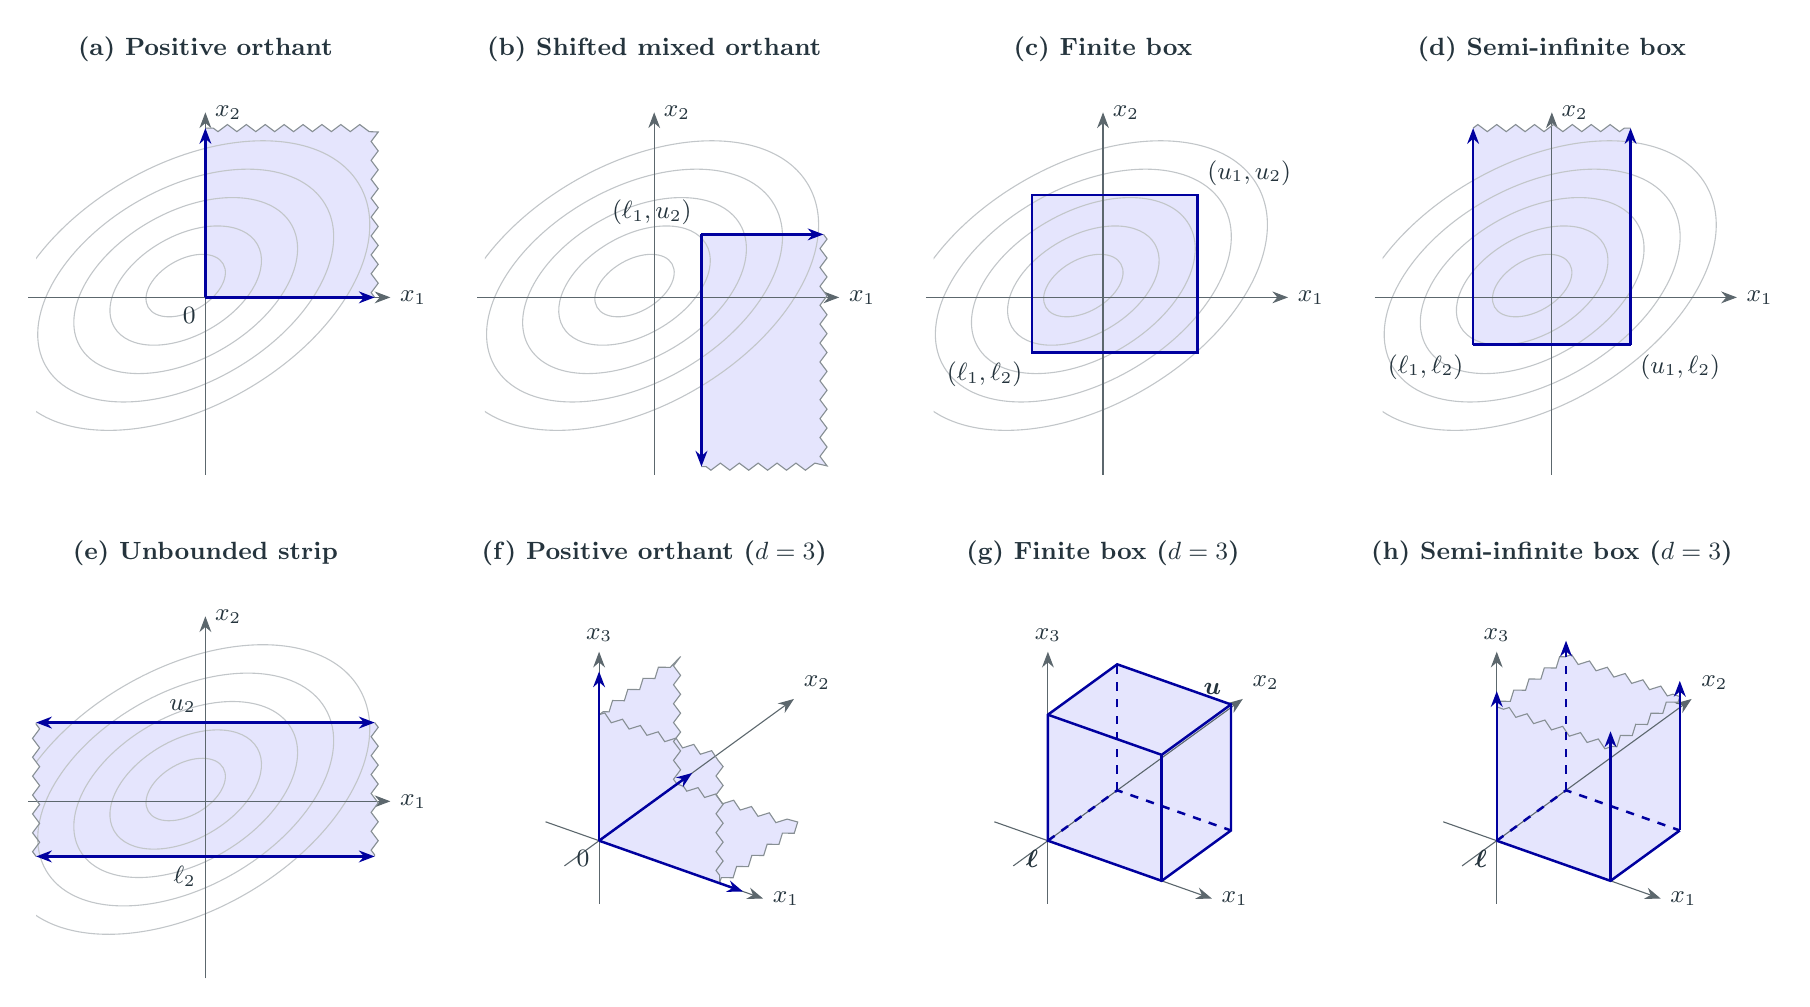
\begin{tikzpicture}
  \begin{scope}[shift={(0.0,0)}]
    \panelheading{(a) Positive orthant}{x_1\geq0,\quad x_2\geq0}
    \fill[fill=shade,sawtooth] (2.15,0)
      decorate {--(2.15,2.15)--(0,2.15)} --(0,0)--cycle;
    \densityaxes
    \draw[continuation] (2.15,0)--(2.15,2.15)--(0,2.15);
    \draw[ray] (0,0)--(2.15,0);
    \draw[ray] (0,0)--(0,2.15);
    \node[label,below left] at (0,0) {$0$};
  \end{scope}

  \begin{scope}[shift={(5.7,0)}]
    \panelheading{(b) Shifted mixed orthant}{x_1\geq\ell_1,\quad x_2\leq u_2}
    \fill[fill=shade,sawtooth] (2.15,0.8)
      decorate {--(2.15,-2.15)--(0.6,-2.15)} --(0.6,0.8)--cycle;
    \densityaxes
    \draw[continuation] (2.15,0.8)--(2.15,-2.15)--(0.6,-2.15);
    \draw[ray] (0.6,0.8)--(2.15,0.8);
    \draw[ray] (0.6,0.8)--(0.6,-2.15);
    \node[label,above left] at (0.6,0.8) {$(\ell_1,u_2)$};
  \end{scope}

  \begin{scope}[shift={(11.4,0)}]
    \panelheading{(c) Finite box}{\ell_1\leq x_1\leq u_1,\quad\ell_2\leq x_2\leq u_2}
    \fill[fill=shade] (-0.9,-0.7) rectangle (1.2,1.3);
    \densityaxes
    \draw[boundary] (-0.9,-0.7) rectangle (1.2,1.3);
    \node[label,below left] at (-0.9,-0.7) {$(\ell_1,\ell_2)$};
    \node[label,above right] at (1.2,1.3) {$(u_1,u_2)$};
  \end{scope}

  \begin{scope}[shift={(17.1,0)}]
    \panelheading{(d) Semi-infinite box}{\ell_1\leq x_1\leq u_1,\quad x_2\geq\ell_2}
    \fill[fill=shade,sawtooth] (-1,2.15)
      decorate {--(1,2.15)} --(1,-0.6)--(-1,-0.6)--cycle;
    \densityaxes
    \draw[continuation] (-1,2.15)--(1,2.15);
    \draw[boundary] (-1,-0.6)--(1,-0.6);
    \draw[ray] (-1,-0.6)--(-1,2.15);
    \draw[ray] (1,-0.6)--(1,2.15);
    \node[label,below left] at (-1,-0.6) {$(\ell_1,\ell_2)$};
    \node[label,below right] at (1,-0.6) {$(u_1,\ell_2)$};
  \end{scope}

  \begin{scope}[shift={(0.0,-6.4)}]
    \panelheading{(e) Unbounded strip}{x_1\in\mathbb{R},\quad\ell_2\leq x_2\leq u_2}
    \fill[fill=shade,sawtooth] (-2.15,-0.7)
      decorate {--(-2.15,1)} --(2.15,1)
      decorate {--(2.15,-0.7)} --cycle;
    \densityaxes
    \draw[continuation] (-2.15,-0.7)--(-2.15,1);
    \draw[continuation] (2.15,1)--(2.15,-0.7);
    \draw[boundary,{Stealth[length=2mm]}-{Stealth[length=2mm]}]
      (-2.15,-0.7)--(2.15,-0.7);
    \draw[boundary,{Stealth[length=2mm]}-{Stealth[length=2mm]}]
      (-2.15,1)--(2.15,1);
    \node[label,below left] at (0,-0.7) {$\ell_2$};
    \node[label,above left] at (0,1) {$u_2$};
  \end{scope}

  \begin{scope}[shift={(5.7,-6.4)}]
    \panelheading{(f) Positive orthant ($d=3$)}{x_i\geq0,\quad i=1,2,3}
    \begin{scope}[shift={(-0.7,-0.5)},
      x={(0.85cm,-0.3cm)},y={(0.55cm,0.4cm)},z={(0cm,1cm)}]
      % Only the three coordinate-plane faces are shaded: there is no upper cap.
      \fill[fill=shade,sawtooth] (1.8,0,0)
        decorate {--(1.8,1.8,0)--(0,1.8,0)} --(0,0,0)--cycle;
      \fill[fill=shade,sawtooth] (0,1.8,0)
        decorate {--(0,1.8,1.6)--(0,0,1.6)} --(0,0,0)--cycle;
      \fill[fill=shade,sawtooth] (0,0,1.6)
        decorate {--(1.8,0,1.6)--(1.8,0,0)} --(0,0,0)--cycle;
      \spaceaxes
      \draw[continuation] (1.8,0,0)--(1.8,1.8,0)--(0,1.8,0);
      \draw[continuation] (0,1.8,0)--(0,1.8,1.6)--(0,0,1.6);
      \draw[continuation] (0,0,1.6)--(1.8,0,1.6)--(1.8,0,0);
      \draw[ray] (0,0,0)--(2.15,0,0);
      \draw[ray] (0,0,0)--(0,2.15,0);
      \draw[ray] (0,0,0)--(0,0,2.15);
      \node[label,below left] at (0,0,0) {$0$};
    \end{scope}
  \end{scope}

  \begin{scope}[shift={(11.4,-6.4)}]
    \panelheading{(g) Finite box ($d=3$)}{\ell_i\leq x_i\leq u_i,\quad i=1,2,3}
    \begin{scope}[shift={(-0.7,-0.5)},
      x={(0.85cm,-0.3cm)},y={(0.55cm,0.4cm)},z={(0cm,1cm)}]
      \fill[fill=shade] (0,0,0)--(1.7,0,0)--(1.7,0,1.6)--(0,0,1.6)--cycle;
      \fill[fill=shade] (1.7,0,0)--(1.7,1.6,0)--(1.7,1.6,1.6)--(1.7,0,1.6)--cycle;
      \fill[fill=shade] (0,0,1.6)--(1.7,0,1.6)--(1.7,1.6,1.6)--(0,1.6,1.6)--cycle;
      \spaceaxes
      % Dashed edges are obscured by the visible faces of the cuboid.
      \draw[boundary,dashed] (0,0,0)--(0,1.6,0)--(1.7,1.6,0);
      \draw[boundary,dashed] (0,1.6,0)--(0,1.6,1.6);
      \draw[boundary] (0,0,0)--(1.7,0,0)--(1.7,1.6,0)--(1.7,1.6,1.6)
        --(0,1.6,1.6)--(0,0,1.6)--cycle;
      \draw[boundary] (0,0,1.6)--(1.7,0,1.6)--(1.7,1.6,1.6);
      \draw[boundary] (1.7,0,0)--(1.7,0,1.6);
      \node[label,below left] at (0,0,0) {$\boldsymbol{\ell}$};
      \node[label,above left] at (1.7,1.6,1.6) {$\boldsymbol{u}$};
    \end{scope}
  \end{scope}

  \begin{scope}[shift={(17.1,-6.4)}]
    \panelheading{(h) Semi-infinite box ($d=3$)}
      {\ell_i\leq x_i\leq u_i\ (i=1,2),\quad x_3\geq\ell_3}
    \begin{scope}[shift={(-0.7,-0.5)},
      x={(0.85cm,-0.3cm)},y={(0.55cm,0.4cm)},z={(0cm,1cm)}]
      % Vertical faces continue upwards; the region has no top face.
      \fill[fill=shade] (0,0,0)--(1.7,0,0)--(1.7,1.6,0)--(0,1.6,0)--cycle;
      % Rear faces parallel to the x_2-x_3 and x_1-x_3 planes.
      \fill[fill=shade,sawtooth] (0,0,1.7)
        decorate {--(0,1.6,1.7)} --(0,1.6,0)--(0,0,0)--cycle;
      \fill[fill=shade,sawtooth] (0,1.6,1.7)
        decorate {--(1.7,1.6,1.7)} --(1.7,1.6,0)--(0,1.6,0)--cycle;
      % Foreground faces, drawn last to preserve the projection order.
      \fill[fill=shade,sawtooth] (1.7,0,1.7)
        decorate {--(0,0,1.7)} --(0,0,0)--(1.7,0,0)--cycle;
      \fill[fill=shade,sawtooth] (1.7,1.6,1.7)
        decorate {--(1.7,0,1.7)} --(1.7,0,0)--(1.7,1.6,0)--cycle;
      \spaceaxes
      \draw[continuation] (0,0,1.7)--(0,1.6,1.7);
      \draw[continuation] (0,1.6,1.7)--(1.7,1.6,1.7);
      \draw[continuation] (1.7,1.6,1.7)--(1.7,0,1.7);
      \draw[continuation] (1.7,0,1.7)--(0,0,1.7);
      \draw[boundary,dashed] (0,0,0)--(0,1.6,0)--(1.7,1.6,0);
      \draw[ray,dashed] (0,1.6,0)--(0,1.6,1.9);
      \draw[boundary] (0,0,0)--(1.7,0,0)--(1.7,1.6,0);
      \draw[ray] (0,0,0)--(0,0,1.9);
      \draw[ray] (1.7,0,0)--(1.7,0,1.9);
      \draw[ray] (1.7,1.6,0)--(1.7,1.6,1.9);
      \node[label,below left] at (0,0,0) {$\boldsymbol{\ell}$};
    \end{scope}
  \end{scope}

\end{tikzpicture}
\end{document}
